\documentclass{amsart}

\usepackage{enumerate, amsmath, amsfonts, amssymb, amsthm, wasysym, graphics, graphicx, xcolor, url, hyperref, hypcap, a4wide, pdflscape, multido, xargs, colortbl, multicol, multirow, calc, shuffle}
\hypersetup{colorlinks=true, citecolor=PineGreen, linkcolor=PineGreen}
%\usepackage[all]{xy}
\usepackage{tikz}\usetikzlibrary{trees,snakes,shapes,arrows,matrix,calc}
\usepackage{comment}
\usepackage{etex}
%\reserveinserts{50}
\graphicspath{{figures/}}
\makeatletter
\def\input@path{{figures/}}
\makeatother

%%%%%%%%%%%%%%%%%%%%%%%%%%%%%%%%%%%%%%

\title{The lattice of acyclic pipe dreams}

\author[N.~Bergeron]{Nantel Bergeron} 
\address[N.~Bergeron]{Department of Mathematics and Statistics, York University, Toronto}
\email{bergeron@yorku.ca}
\urladdr{http://bergeron.mathstats.yorku.ca}

\author[N.~Cartier]{No\'emie Cartier} 
\address[N.~Cartier]{LRI, Université Paris Saclay}
\email{noemie.cartier@lri.fr}

\author[C.~Ceballos]{Cesar Ceballos}
\address[C.~Ceballos]{Institute of Geometry, Technische Universit\"at Graz}
\email{cesar.ceballos@tugraz.at}
\urladdr{http://www.geometrie.tugraz.at/ceballos/}

\author[V.~Pilaud]{Vincent Pilaud}
\address[V.~Pilaud]{CNRS \& LIX, \'Ecole Polytechnique, Palaiseau}
\email{vincent.pilaud@lix.polytechnique.fr}
\urladdr{http://www.lix.polytechnique.fr/~pilaud/}

%%%%%%%%%%%%%%%%%%%%%%%%%%%%%%%%%%%%%%

% theorems
\newtheorem{theorem}{Theorem}%[section]
\newtheorem{corollary}[theorem]{Corollary}
\newtheorem{proposition}[theorem]{Proposition}
\newtheorem{lemma}[theorem]{Lemma}
\newtheorem{definition}[theorem]{Definition}
\newtheorem{conjecture}[theorem]{Conjecture}

\theoremstyle{definition}
\newtheorem{example}[theorem]{Example}
\newtheorem{remark}[theorem]{Remark}
\newtheorem{question}[theorem]{Question}

% newcommands
% math special letters
\newcommand{\R}{\mathbb{R}} % reals
\newcommand{\N}{\mathbb{N}} % naturals
\newcommand{\Z}{\mathbb{Z}} % integers
\newcommand{\I}{\mathbb{I}} % set of integers
\newcommand{\C}{\mathbb{C}} % set of summands

% math commands
\newcommand{\set}[2]{\left\{ #1 \;\middle|\; #2 \right\}} % set notation
\newcommand{\bigset}[2]{\big\{ #1 \;|\; #2 \big\}} % big set notation
\newcommand{\biggset}[2]{\bigg\{ #1 \;\bigg|\; #2 \bigg\}} % big set notation
\newcommand{\multiset}[2]{\left\{\!\!\left\{ #1 \;\middle|\; #2 \right\}\!\!\right\}} % multiset notation
\newcommand{\bigmultiset}[2]{\big\{\!\!\big\{ #1 \;|\; #2 \big\}\!\!\big\}} % big multiset notation
\newcommand{\ssm}{\smallsetminus} % small set minus
\newcommand{\dotprod}[2]{\langle #1 | #2 \rangle} % dot product
\newcommand{\symdif}{\triangle} % symmetric difference
\newcommand{\one}{{1\!\!1}} % the all one vector
\newcommand{\eqdef}{\mbox{\,\raisebox{0.2ex}{\scriptsize\ensuremath{\mathrm:}}\ensuremath{=}\,}} % :=
\newcommand{\defeq}{\mbox{~\ensuremath{=}\raisebox{0.2ex}{\scriptsize\ensuremath{\mathrm:}} }} % =:
\newcommand{\polar}{^\diamond} % polar
\newcommand{\simplex}{\triangle} % simplex

% operators
\DeclareMathOperator{\conv}{conv} % convex hull
\DeclareMathOperator{\cone}{cone} % cone hull
\DeclareMathOperator{\arr}{Arr} % arrangements
\DeclareMathOperator{\inv}{inv} % inversion set

% others
\newcommand{\fix}[1]{{\bf FIXME: }#1} % emphasis of a problem to FIX
\newcommand{\fref}[1]{Figure~\ref{#1}} % reference figures
\newcommand{\ie}{\textit{i.e.}~} % id est
\newcommand{\eg}{\textit{e.g.}~} % exempli gratia
\newcommand{\Eg}{\textit{E.g.}~} % exempli gratia
\newcommand{\aka}{\textit{aka.}~} % also known as
\newcommand{\viceversa}{\textit{vice versa}} % vice versa
\newcommand{\ordinal}{\textsuperscript{th}} % th for ordinals
\newcommand{\ex}[1]{^{\textrm{ex#1}}} % example
\newcommand{\para}[1]{\medskip\noindent\textbf{#1~---}} % paragraph
\newcommand{\subpara}[1]{\smallskip\noindent\textit{#1.}} % paragraph
\definecolor{PineGreen}{RGB}{2,120,120} % pinegreen color
\definecolor{darkgreen}{RGB}{57,181,74} % darkgreen color
\renewcommand{\b}[1]{{\color{blue} #1}} % blue
\renewcommand{\r}[1]{{\color{red} #1}} % red
\newcommand{\g}[1]{{\color{darkgreen} #1}} % green
\newcommand{\defn}[1]{\textbf{\textsf{\color{PineGreen} #1}}} % emphasis of a definition
\usepackage{todonotes}
\newcommand{\nantel}[1]{\todo[color=red!30]{#1 \\ \hfill --- N.}}
\newcommand{\cesar}[1]{\todo[color=orange!30]{#1 \\ \hfill --- C.}}
\newcommand{\noemie}[1]{\todo[color=green!30]{#1 \\ \hfill --- N.}}
\newcommand{\vincent}[1]{\todo[color=blue!30]{#1 \\ \hfill --- V.}}

% permutations
\newcommand{\fS}{\mathfrak{S}} % symmetric group
\newcommand{\gdproduct}{\bullet} % global descent product
\newcommand{\gdshuffle}{\shuffle_\gdproduct} % global descent shuffle product
\newcommand{\gddeconcat}{\coproduct_\gdproduct} % global descent deconcatenation coproduct
\newcommand{\HS}{{\bk\fS}} % Hopf Algebra of permutations
\newcommand{\shiftedShuffle}{\,\bar\shuffle\,} % shifted shuffle
\newcommand{\convolution}{\star} % convolution

% pipe dreams
\newcommand{\boxsize}{.35}
\newlength{\verticalOffset}
\setlength{\verticalOffset}{.3cm}
\newlength{\verticalShift}
\setlength{\verticalShift}{-.15cm}

\newcounter{length}
\newcommand{\length}[1]{%
	\setcounter{length}{0}%
	\foreach \x in {#1} {%
		\stepcounter{length}%
	}%
}

\newcommand{\pipeDreamMonoColor}[3]{% #1 = color
									% #2 = boundary color
                                    % #3 = list of types (c = cross, e = elbow, t = top, b = bottom, tb = top-bottom, or n = nothing)
	\length{#3}%
	\begin{tikzpicture}[baseline = \value{length}*\verticalShift+\verticalOffset, scale=1]
		\coordinate (origin) at (0,0);
		\newcount{\y} \y=0
		\newcount{\x}
		\foreach \line in {#3} {
			\x=0
			\foreach \t in \line {
				\coordinate (W) at ($ (origin) + ( \boxsize * \x , -\boxsize * \y ) + ( 0      , \boxsize / 2 ) $);
				\coordinate (E) at ($ (origin) + ( \boxsize * \x , -\boxsize * \y ) + ( \boxsize     , \boxsize / 2 ) $);
				\coordinate (N) at ($ (origin) + ( \boxsize * \x , -\boxsize * \y ) + ( \boxsize / 2 , \boxsize     ) $);
				\coordinate (S) at ($ (origin) + ( \boxsize * \x , -\boxsize * \y ) + ( \boxsize / 2 , 0 ) $);
				\coordinate (C) at ($ (origin) + ( \boxsize * \x , -\boxsize * \y ) + ( \boxsize / 2 , \boxsize / 2 ) $);
				\ifthenelse{\equal{\t}{e}}{
					\draw[rounded corners=\boxsize * 8, color=#1, thick] (W) -- (C) -- (N);
					\draw[rounded corners=\boxsize * 8, color=#1, thick] (S) -- (C) -- (E);			
				}{
        				\ifthenelse{\equal{\t}{c}}{
        					\draw[color=#1, thick] (W) -- (E);
        					\draw[color=#1, thick] (S) -- (N);
        				}{
        				\ifthenelse{\equal{\t}{t}}{
        					\draw[rounded corners=\boxsize * 8, color=#2] (W) -- (C) -- (N);
        					\draw[rounded corners=\boxsize * 8, color=#1, thick] (S) -- (C) -- (E);			
        				}{
        				\ifthenelse{\equal{\t}{b}}{
        					\draw[rounded corners=\boxsize * 8, color=#1, thick] (W) -- (C) -- (N);
        					\draw[rounded corners=\boxsize * 8, color=#2] (S) -- (C) -- (E);			
        				}{
        				\ifthenelse{\equal{\t}{tb}}{
        					\draw[rounded corners=\boxsize * 8, color=#2] (W) -- (C) -- (N);
        					\draw[rounded corners=\boxsize * 8, color=#2] (S) -- (C) -- (E);			
        				}{
        				\ifthenelse{\equal{\t}{n}}{}{\node at (C) {$\small \t$};}}}}}}
        				\global\advance\x by 1
			}
			\global\advance\y by 1
		}
	\end{tikzpicture}%
}

\newcommand{\pipeDreamBiColor}[4]{% #1 = colorA
                                   % #2 = colorB
                                   % #3 = boundary color
                                   % #4 = list of type/colorW/colorS (c = cross, e = elbow, or n = nothing)
	\length{#4}%
	\begin{tikzpicture}[baseline = \value{length}*\verticalShift+\verticalOffset, scale=1]
		\coordinate (origin) at (0,0);
		\newcount{\y} \y=0
		\newcount{\x}
		\foreach \line in {#4} {
			\x=0
			\foreach \t/\colorW/\colorS in \line {
				\coordinate (W) at ($ (origin) + ( \boxsize * \x , -\boxsize * \y ) + ( 0      , \boxsize / 2 ) $);
				\coordinate (E) at ($ (origin) + ( \boxsize * \x , -\boxsize * \y ) + ( \boxsize     , \boxsize / 2 ) $);
				\coordinate (N) at ($ (origin) + ( \boxsize * \x , -\boxsize * \y ) + ( \boxsize / 2 , \boxsize     ) $);
				\coordinate (S) at ($ (origin) + ( \boxsize * \x , -\boxsize * \y ) + ( \boxsize / 2 , 0 ) $);
				\coordinate (C) at ($ (origin) + ( \boxsize * \x , -\boxsize * \y ) + ( \boxsize / 2 , \boxsize / 2 ) $);
				\ifthenelse{\equal{\t}{e}}{
					\ifthenelse{\equal{\colorW}{l}}{\draw[rounded corners=\boxsize * 8, color=#1, thick] (W) -- (C) -- (N);}{}
					\ifthenelse{\equal{\colorW}{r}}{\draw[rounded corners=\boxsize * 8, color=#2, thick] (W) -- (C) -- (N);}{}
					\ifthenelse{\equal{\colorW}{b}}{\draw[rounded corners=\boxsize * 8, color=#3] (W) -- (C) -- (N);}{}
					\ifthenelse{\equal{\colorS}{l}}{\draw[rounded corners=\boxsize * 8, color=#1, thick] (S) -- (C) -- (E);}{}
					\ifthenelse{\equal{\colorS}{r}}{\draw[rounded corners=\boxsize * 8, color=#2, thick] (S) -- (C) -- (E);}{}
					\ifthenelse{\equal{\colorS}{b}}{\draw[rounded corners=\boxsize * 8, color=#3] (S) -- (C) -- (E);}{}
				}{
				\ifthenelse{\equal{\t}{c}}{
					\ifthenelse{\equal{\colorW}{l}}{\draw[color=#1, thick] (W) -- (E);}{}
					\ifthenelse{\equal{\colorW}{r}}{\draw[color=#2, thick] (W) -- (E);}{}
					\ifthenelse{\equal{\colorS}{l}}{\draw[color=#1, thick] (S) -- (N);}{}
					\ifthenelse{\equal{\colorS}{r}}{\draw[color=#2, thick] (S) -- (N);}{}
				}{
				\ifthenelse{\equal{\t}{n}}{}{\node at (C) {$\small \t$};}}}
				\global\advance\x by 1
			}
			\global\advance\y by 1
		}
	\end{tikzpicture}%
}

\newcommand{\pipeDreamTriColor}[5]{% #1 = colorA
                                   % #2 = colorB
                                   % #3 = colorC
                                   % #4 = boundary color
                                   % #5 = list of type/colorW/colorS (c = cross, e = elbow, or n = nothing)
	\length{#5}%
	\begin{tikzpicture}[baseline = \value{length}*\verticalShift+\verticalOffset, scale=1]
		\coordinate (origin) at (0,0);
		\newcount{\y} \y=0
		\newcount{\x}
		\foreach \line in {#5} {
			\x=0
			\foreach \t/\colorW/\colorS in \line {
				\coordinate (W) at ($ (origin) + ( \boxsize * \x , -\boxsize * \y ) + ( 0      , \boxsize / 2 ) $);
				\coordinate (E) at ($ (origin) + ( \boxsize * \x , -\boxsize * \y ) + ( \boxsize     , \boxsize / 2 ) $);
				\coordinate (N) at ($ (origin) + ( \boxsize * \x , -\boxsize * \y ) + ( \boxsize / 2 , \boxsize     ) $);
				\coordinate (S) at ($ (origin) + ( \boxsize * \x , -\boxsize * \y ) + ( \boxsize / 2 , 0 ) $);
				\coordinate (C) at ($ (origin) + ( \boxsize * \x , -\boxsize * \y ) + ( \boxsize / 2 , \boxsize / 2 ) $);
				\ifthenelse{\equal{\t}{e}}{
					\ifthenelse{\equal{\colorW}{l}}{\draw[rounded corners=\boxsize * 8, color=#1, thick] (W) -- (C) -- (N);}{}
					\ifthenelse{\equal{\colorW}{m}}{\draw[rounded corners=\boxsize * 8, color=#2, thick] (W) -- (C) -- (N);}{}
					\ifthenelse{\equal{\colorW}{r}}{\draw[rounded corners=\boxsize * 8, color=#3, thick] (W) -- (C) -- (N);}{}
					\ifthenelse{\equal{\colorW}{b}}{\draw[rounded corners=\boxsize * 8, color=#4] (W) -- (C) -- (N);}{}
					\ifthenelse{\equal{\colorS}{l}}{\draw[rounded corners=\boxsize * 8, color=#1, thick] (S) -- (C) -- (E);}{}
					\ifthenelse{\equal{\colorS}{m}}{\draw[rounded corners=\boxsize * 8, color=#2, thick] (S) -- (C) -- (E);}{}
					\ifthenelse{\equal{\colorS}{r}}{\draw[rounded corners=\boxsize * 8, color=#3, thick] (S) -- (C) -- (E);}{}
					\ifthenelse{\equal{\colorS}{b}}{\draw[rounded corners=\boxsize * 8, color=#4] (S) -- (C) -- (E);}{}
				}{
				\ifthenelse{\equal{\t}{c}}{
					\ifthenelse{\equal{\colorW}{l}}{\draw[color=#1, thick] (W) -- (E);}{}
					\ifthenelse{\equal{\colorW}{m}}{\draw[color=#2, thick] (W) -- (E);}{}
					\ifthenelse{\equal{\colorW}{r}}{\draw[color=#3, thick] (W) -- (E);}{}
					\ifthenelse{\equal{\colorS}{l}}{\draw[color=#1, thick] (S) -- (N);}{}
					\ifthenelse{\equal{\colorS}{m}}{\draw[color=#2, thick] (S) -- (N);}{}
					\ifthenelse{\equal{\colorS}{r}}{\draw[color=#3, thick] (S) -- (N);}{}
				}{\ifthenelse{\equal{\t}{n}}{}{\node at (C) {$\small \t$};}}}
				\global\advance\x by 1
			}
			\global\advance\y by 1
		}
	\end{tikzpicture}%
}

%\newcommand{\pipeDreamBiColor}[4]{% #1 = colorA
%                                  % #2 = colorB
%                                  % #3 = boundary color
%                                  % #4 = list of type/colorW/colorS (c = cross, e = elbow, t = top, b = bottom, tb = top-bottom, or n = nothing)
%	\length{#4}%
%	\begin{tikzpicture}[baseline = \value{length}*\verticalShift+\verticalOffset, scale=1]
%		\coordinate (origin) at (0,0);
%		\newcount{\y} \y=0
%		\newcount{\x}
%		\foreach \line in {#4} {
%			\x=0
%			\foreach \t/\colorW/\colorS in \line {
%				\coordinate (W) at ($ (origin) + ( \boxsize * \x , -\boxsize * \y ) + ( 0      , \boxsize / 2 ) $);
%				\coordinate (E) at ($ (origin) + ( \boxsize * \x , -\boxsize * \y ) + ( \boxsize     , \boxsize / 2 ) $);
%				\coordinate (N) at ($ (origin) + ( \boxsize * \x , -\boxsize * \y ) + ( \boxsize / 2 , \boxsize     ) $);
%				\coordinate (S) at ($ (origin) + ( \boxsize * \x , -\boxsize * \y ) + ( \boxsize / 2 , 0 ) $);
%				\coordinate (C) at ($ (origin) + ( \boxsize * \x , -\boxsize * \y ) + ( \boxsize / 2 , \boxsize / 2 ) $);
%				\ifthenelse{\equal{\t}{e}}{
%					\ifthenelse{\equal{\colorW}{l}}{\draw[rounded corners=\boxsize * 8, color=#1, thick] (W) -- (C) -- (N);}{\draw[rounded corners=\boxsize * 8, color=#2, thick] (W) -- (C) -- (N);}
%					\ifthenelse{\equal{\colorS}{l}}{\draw[rounded corners=\boxsize * 8, color=#1, thick] (S) -- (C) -- (E);}{\draw[rounded corners=\boxsize * 8, color=#2, thick] (S) -- (C) -- (E);}
%				}{}
%				\ifthenelse{\equal{\t}{c}}{
%					\ifthenelse{\equal{\colorW}{l}}{\draw[color=#1, thick] (W) -- (E);}{\draw[color=#2, thick] (W) -- (E);}
%					\ifthenelse{\equal{\colorS}{l}}{\draw[color=#1, thick] (S) -- (N);}{\draw[color=#2, thick] (S) -- (N);}
%				}{}
%				\ifthenelse{\equal{\t}{t}}{
%					\ifthenelse{\equal{\colorW}{l}}{\draw[rounded corners=\boxsize * 8, color=#1] (W) -- (C) -- (N);}{}
%					\ifthenelse{\equal{\colorW}{r}}{\draw[rounded corners=\boxsize * 8, color=#2] (W) -- (C) -- (N);}{}
%					\ifthenelse{\equal{\colorW}{b}}{\draw[rounded corners=\boxsize * 8, color=#3] (W) -- (C) -- (N);}{}
%					\ifthenelse{\equal{\colorS}{l}}{\draw[rounded corners=\boxsize * 8, color=#1, thick] (S) -- (C) -- (E);}{\draw[rounded corners=\boxsize * 8, color=#2, thick] (S) -- (C) -- (E);}
%				}{}
%				\ifthenelse{\equal{\t}{b}}{
%					\ifthenelse{\equal{\colorW}{l}}{\draw[rounded corners=\boxsize * 8, color=#1, thick] (W) -- (C) -- (N);}{\draw[rounded corners=\boxsize * 8, color=#2, thick] (W) -- (C) -- (N);}
%					\ifthenelse{\equal{\colorS}{l}}{\draw[rounded corners=\boxsize * 8, color=#1] (S) -- (C) -- (E);}{}
%					\ifthenelse{\equal{\colorS}{r}}{\draw[rounded corners=\boxsize * 8, color=#2] (S) -- (C) -- (E);}{}
%					\ifthenelse{\equal{\colorS}{b}}{\draw[rounded corners=\boxsize * 8, color=#3] (S) -- (C) -- (E);}{}
%				}{}
%				\ifthenelse{\equal{\t}{tb}}{
%					\ifthenelse{\equal{\colorW}{l}}{\draw[rounded corners=\boxsize * 8, color=#1] (W) -- (C) -- (N);}{}
%					\ifthenelse{\equal{\colorW}{r}}{\draw[rounded corners=\boxsize * 8, color=#2] (W) -- (C) -- (N);}{}
%					\ifthenelse{\equal{\colorW}{b}}{\draw[rounded corners=\boxsize * 8, color=#3] (W) -- (C) -- (N);}{}
%					\ifthenelse{\equal{\colorS}{l}}{\draw[rounded corners=\boxsize * 8, color=#1] (S) -- (C) -- (E);}{}
%					\ifthenelse{\equal{\colorS}{r}}{\draw[rounded corners=\boxsize * 8, color=#2] (S) -- (C) -- (E);}{}
%					\ifthenelse{\equal{\colorS}{b}}{\draw[rounded corners=\boxsize * 8, color=#3] (S) -- (C) -- (E);}{}
%				}{}
%				\global\advance\x by 1
%			}
%			\global\advance\y by1
%		}
%	\end{tikzpicture}%
%}
% cross
%\newcommand{\cross}[1][black]{\raisebox{.1cm}{\pipeDreamMonoColor{#1}{black}{c}}}
\newcommand{\cross}[1][black]{\raisebox{-.15cm}{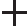
\includegraphics[scale=.9]{cross}}}
\newcommand{\crossBiColor}[2]{\raisebox{.1cm}{\pipeDreamBiColor{#1}{#2}{black}{c/l/r}}}
\newcommand{\NScross}[1][black]{\raisebox{-.15cm}{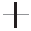
\includegraphics[scale=.9]{NScross}}}
\newcommand{\WEcross}[1][black]{\raisebox{-.15cm}{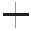
\includegraphics[scale=.9]{WEcross}}}
% elbow
%\newcommand{\elbow}[1][black]{\raisebox{.1cm}{\pipeDreamMonoColor{#1}{black}{e}}}
\newcommand{\elbow}[1][black]{\raisebox{-.15cm}{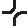
\includegraphics[scale=.9]{elbow}}}
\newcommand{\elbowBiColor}[2]{\raisebox{.1cm}{\pipeDreamBiColor{#1}{#2}{black}{e/l/r}}}
%\newcommand{\SEelbow}[1][black]{\raisebox{.1cm}{\pipeDreamBiColor{white}{#1}{black}{e/l/r}}}
\newcommand{\SEelbow}[1][black]{\raisebox{-.15cm}{
\includegraphics[scale=.9]{SEelbow}}}
%\newcommand{\WNelbow}[1][black]{\raisebox{.1cm}{\pipeDreamBiColor{#1}{white}{black}{e/l/r}}}
\newcommand{\WNelbow}[1][black]{\raisebox{-.15cm}{
\includegraphics[scale=.9]{WNelbow}}}
\newcommand{\waving}{\mathsf{wav}}%{\raisebox{-.2cm}{\begin{tikzpicture}[scale=1]\pipeDreamBiColor{.2}{(0,0)}{black}{white}{{t/r/l},{t/l/l},{t/l/r}}\end{tikzpicture}}}
\newcommand{\transpose}{\mathsf{transp}}
\newcommand{\pipeDreams}{\Pi} % set of pipe dreams
\newcommand{\HP}{{\bk\pipeDreams}} % Hopf Algebra of pipe dreams
\newcommand{\reversingPipeDreams}{\Omega} % reversing pipe dreams
\newcommand{\contact}{^\#} % contact graph
\newcommand{\se}{\textsc{se}} % south-east
\newcommand{\nw}{\textsc{nw}} % north-west
\newcommand{\insertion}[2]{\mathsf{ins}(#1,#2)} % insertion of permutation #1 in pipe dreams with permutation #2
\newcommand{\duality}{^\star} % duality pipe dreams - triangulations
\newcommand{\acyclicPipeDreams}{\Sigma} % acyclic pipe dreams
\newcommand{\wo}{w_\circ} % longest element
\newcommand{\subwordComplex}{\mathcal{SC}} % subword complex
\newcommand{\Roots}{\mathrm{R}} % root configuration
\newcommand{\linearExtensions}{\mathcal{L}} % linear extensions
\newcommand{\noninversions}[2]{\mathsf{ninv}(#1,#2)} % non-inversions
\newcommand{\acyclicOrientations}{\Omega} % set of pipe dreams
\newcommand{\recoils}[2]{\mathsf{rec}(#1,#2)} % recoil scheme of a pipe dream
\newcommand{\canopy}[1]{\mathsf{can}(#1)} % canopy of a pipe dream

% lattices
\newcommand{\meet}{\wedge} % meet
\newcommand{\join}{\vee} % join
\newcommand{\less}{\vartriangleleft} % smaller WOIP
\newcommand{\more}{\vartriangleright} % larger WOIP
\newcommand{\contactLess}[1]{\less_{#1}} % smaller contact graph
\newcommand{\contactMore}[1]{\more_{#1}} % larger contact graph
\newcommand{\projDown}{\pi_\downarrow} % Down projection
\newcommand{\projUp}{\pi^\uparrow} % Down projection


%%%%%%%%%%%%%%%%%%%%%%%%%%%%%%%%%%%%%%
%%%%%%%%%%%%%%%%%%%%%%%%%%%%%%%%%%%%%%
%%%%%%%%%%%%%%%%%%%%%%%%%%%%%%%%%%%%%%

\begin{document}

\begin{abstract}
We show that for any permutation~$\omega$, the increasing flip graph on acyclic pipe dreams with permutation~$\omega$ is a lattice quotient of the interval~$[e,\omega]$ of the weak order.
\end{abstract}

\maketitle

%%%%%%%%%%%%%%%%%%%%%%%%%%%%%%%%%%%%%%
%%%%%%%%%%%%%%%%%%%%%%%%%%%%%%%%%%%%%%
%%%%%%%%%%%%%%%%%%%%%%%%%%%%%%%%%%%%%%

The purpose of this note is to show that for any permutation~$\omega$, the increasing flip graph on acyclic pipe dreams with permutation~$\omega$ is a lattice quotient of the interval~$[e,\omega]$ of the weak order. It motivates Conjecture~\ref{conj:Coxeter} which is the long-term perspective of this work. The approach and proofs developed here are direct adaptations from~\cite[Sect.~1]{Pilaud-BrickAlgebra}.

\section{Preliminaries}
\label{sec:preliminaries}

% Let $\fS_n$ denote the set of permutations of~$[n] \eqdef \{1,2,\ldots,n\}$, and let~$\fS \eqdef \bigsqcup_{n \ge 0} \fS_n$.

%%%%%%%%%%%%%%%%%%%%%%%%%%%%%%%%%%%%%%

\subsection{Pipe dreams}
\label{subsec:pipeDreams}

A \defn{pipe dream}~$P$ is a filling of a triangular shape with crosses~\cross{} and elbows~\elbow{} so that all pipes entering on the left side exit on the top side. We only consider \defn{reduced} pipe dreams, where two pipes have at most one intersection. We label the pipes with~$1, 2, \dots, n$ in the order of their entry points from top to bottom. We denote by~$\omega_P \in \fS_n$ the order of the exit points of the non-zero pipes of~$P$ from left to right. In other words, the pipe entering at row~$i$ exits at column~$\omega^{-1}_P(i)$. For a fixed permutation~$\omega \in \fS_n$, we denote by~$\pipeDreams(\omega)$ the set of reduced pipe dreams~$P$ such that~$\omega_P = \omega$.
% We let~$\pipeDreams_n \eqdef \bigsqcup_{\omega \in \fS_n} \pipeDreams(\omega)$ and~$\pipeDreams \eqdef \bigsqcup_{n \in \N} \pipeDreams_n$. 

\begin{figure}[ht]
	\centerline{
		%\documentclass[10pt]{article}
\usepackage[usenames]{color} %pour la couleur
\usepackage{amssymb} %maths
\usepackage{amsmath} %maths
\usepackage[utf8]{inputenc} %utile pour taper directement les caractères accentués
\usepackage{tikz}\usetikzlibrary{trees,snakes,shapes,arrows,matrix,calc}
\usepackage{pgfplots}
\usepackage{xifthen}
\usepackage{xcolor}
\definecolor{darkgreen}{RGB}{57,181,74} % darkgreen color

\renewcommand{\b}[1]{{\color{blue} #1}} % blue
\renewcommand{\r}[1]{{\color{red} #1}} % red
\newcommand{\g}[1]{{\color{darkgreen} #1}} % green

\newcommand{\boxsize}{.35}
\newlength{\verticalOffset}
\setlength{\verticalOffset}{.3cm}
\newlength{\verticalShift}
\setlength{\verticalShift}{-.15cm}

\newcounter{length}
\newcommand{\length}[1]{%
	\setcounter{length}{0}%
	\foreach \x in {#1} {%
		\stepcounter{length}%
	}%
}

\newcommand{\pipeDreamMonoColor}[3]{% #1 = color
									% #2 = boundary color
                                    % #3 = list of types (c = cross, e = elbow, t = top, b = bottom, tb = top-bottom, or n = nothing)
	\length{#3}%
	\begin{tikzpicture}[baseline = \value{length}*\verticalShift+\verticalOffset, scale=1]
		\coordinate (origin) at (0,0);
		\newcount{\y} \y=0
		\newcount{\x}
		\foreach \line in {#3} {
			\x=0
			\foreach \t in \line {
				\coordinate (W) at ($ (origin) + ( \boxsize * \x , -\boxsize * \y ) + ( 0      , \boxsize / 2 ) $);
				\coordinate (E) at ($ (origin) + ( \boxsize * \x , -\boxsize * \y ) + ( \boxsize     , \boxsize / 2 ) $);
				\coordinate (N) at ($ (origin) + ( \boxsize * \x , -\boxsize * \y ) + ( \boxsize / 2 , \boxsize     ) $);
				\coordinate (S) at ($ (origin) + ( \boxsize * \x , -\boxsize * \y ) + ( \boxsize / 2 , 0 ) $);
				\coordinate (C) at ($ (origin) + ( \boxsize * \x , -\boxsize * \y ) + ( \boxsize / 2 , \boxsize / 2 ) $);
				\ifthenelse{\equal{\t}{e}}{
					\draw[rounded corners=\boxsize * 8, color=#1, thick] (W) -- (C) -- (N);
					\draw[rounded corners=\boxsize * 8, color=#1, thick] (S) -- (C) -- (E);			
				}{
        				\ifthenelse{\equal{\t}{c}}{
        					\draw[color=#1, thick] (W) -- (E);
        					\draw[color=#1, thick] (S) -- (N);
        				}{
        				\ifthenelse{\equal{\t}{t}}{
        					\draw[rounded corners=\boxsize * 8, color=#2] (W) -- (C) -- (N);
        					\draw[rounded corners=\boxsize * 8, color=#1, thick] (S) -- (C) -- (E);			
        				}{
        				\ifthenelse{\equal{\t}{b}}{
        					\draw[rounded corners=\boxsize * 8, color=#1, thick] (W) -- (C) -- (N);
        					\draw[rounded corners=\boxsize * 8, color=#2] (S) -- (C) -- (E);			
        				}{
        				\ifthenelse{\equal{\t}{tb}}{
        					\draw[rounded corners=\boxsize * 8, color=#2] (W) -- (C) -- (N);
        					\draw[rounded corners=\boxsize * 8, color=#2] (S) -- (C) -- (E);			
        				}{
        				\ifthenelse{\equal{\t}{n}}{}{\node at (C) {$\small \t$};}}}}}}
        				\global\advance\x by 1
			}
			\global\advance\y by 1
		}
	\end{tikzpicture}%
}

\newcommand{\pipeDreamBiColor}[4]{% #1 = colorA
                                   % #2 = colorB
                                   % #3 = boundary color
                                   % #4 = list of type/colorW/colorS (c = cross, e = elbow, or n = nothing)
	\length{#4}%
	\begin{tikzpicture}[baseline = \value{length}*\verticalShift+\verticalOffset, scale=1]
		\coordinate (origin) at (0,0);
		\newcount{\y} \y=0
		\newcount{\x}
		\foreach \line in {#4} {
			\x=0
			\foreach \t/\colorW/\colorS in \line {
				\coordinate (W) at ($ (origin) + ( \boxsize * \x , -\boxsize * \y ) + ( 0      , \boxsize / 2 ) $);
				\coordinate (E) at ($ (origin) + ( \boxsize * \x , -\boxsize * \y ) + ( \boxsize     , \boxsize / 2 ) $);
				\coordinate (N) at ($ (origin) + ( \boxsize * \x , -\boxsize * \y ) + ( \boxsize / 2 , \boxsize     ) $);
				\coordinate (S) at ($ (origin) + ( \boxsize * \x , -\boxsize * \y ) + ( \boxsize / 2 , 0 ) $);
				\coordinate (C) at ($ (origin) + ( \boxsize * \x , -\boxsize * \y ) + ( \boxsize / 2 , \boxsize / 2 ) $);
				\ifthenelse{\equal{\t}{e}}{
					\ifthenelse{\equal{\colorW}{l}}{\draw[rounded corners=\boxsize * 8, color=#1, thick] (W) -- (C) -- (N);}{}
					\ifthenelse{\equal{\colorW}{r}}{\draw[rounded corners=\boxsize * 8, color=#2, thick] (W) -- (C) -- (N);}{}
					\ifthenelse{\equal{\colorW}{b}}{\draw[rounded corners=\boxsize * 8, color=#3] (W) -- (C) -- (N);}{}
					\ifthenelse{\equal{\colorS}{l}}{\draw[rounded corners=\boxsize * 8, color=#1, thick] (S) -- (C) -- (E);}{}
					\ifthenelse{\equal{\colorS}{r}}{\draw[rounded corners=\boxsize * 8, color=#2, thick] (S) -- (C) -- (E);}{}
					\ifthenelse{\equal{\colorS}{b}}{\draw[rounded corners=\boxsize * 8, color=#3] (S) -- (C) -- (E);}{}
				}{
				\ifthenelse{\equal{\t}{c}}{
					\ifthenelse{\equal{\colorW}{l}}{\draw[color=#1, thick] (W) -- (E);}{}
					\ifthenelse{\equal{\colorW}{r}}{\draw[color=#2, thick] (W) -- (E);}{}
					\ifthenelse{\equal{\colorS}{l}}{\draw[color=#1, thick] (S) -- (N);}{}
					\ifthenelse{\equal{\colorS}{r}}{\draw[color=#2, thick] (S) -- (N);}{}
				}{
				\ifthenelse{\equal{\t}{n}}{}{\node at (C) {$\small \t$};}}}
				\global\advance\x by 1
			}
			\global\advance\y by 1
		}
	\end{tikzpicture}%
}

\newcommand{\pipeDreamTriColor}[5]{% #1 = colorA
                                   % #2 = colorB
                                   % #3 = colorC
                                   % #4 = boundary color
                                   % #5 = list of type/colorW/colorS (c = cross, e = elbow, or n = nothing)
	\length{#5}%
	\begin{tikzpicture}[baseline = \value{length}*\verticalShift+\verticalOffset, scale=1]
		\coordinate (origin) at (0,0);
		\newcount{\y} \y=0
		\newcount{\x}
		\foreach \line in {#5} {
			\x=0
			\foreach \t/\colorW/\colorS in \line {
				\coordinate (W) at ($ (origin) + ( \boxsize * \x , -\boxsize * \y ) + ( 0      , \boxsize / 2 ) $);
				\coordinate (E) at ($ (origin) + ( \boxsize * \x , -\boxsize * \y ) + ( \boxsize     , \boxsize / 2 ) $);
				\coordinate (N) at ($ (origin) + ( \boxsize * \x , -\boxsize * \y ) + ( \boxsize / 2 , \boxsize     ) $);
				\coordinate (S) at ($ (origin) + ( \boxsize * \x , -\boxsize * \y ) + ( \boxsize / 2 , 0 ) $);
				\coordinate (C) at ($ (origin) + ( \boxsize * \x , -\boxsize * \y ) + ( \boxsize / 2 , \boxsize / 2 ) $);
				\ifthenelse{\equal{\t}{e}}{
					\ifthenelse{\equal{\colorW}{l}}{\draw[rounded corners=\boxsize * 8, color=#1, thick] (W) -- (C) -- (N);}{}
					\ifthenelse{\equal{\colorW}{m}}{\draw[rounded corners=\boxsize * 8, color=#2, thick] (W) -- (C) -- (N);}{}
					\ifthenelse{\equal{\colorW}{r}}{\draw[rounded corners=\boxsize * 8, color=#3, thick] (W) -- (C) -- (N);}{}
					\ifthenelse{\equal{\colorW}{b}}{\draw[rounded corners=\boxsize * 8, color=#4] (W) -- (C) -- (N);}{}
					\ifthenelse{\equal{\colorS}{l}}{\draw[rounded corners=\boxsize * 8, color=#1, thick] (S) -- (C) -- (E);}{}
					\ifthenelse{\equal{\colorS}{m}}{\draw[rounded corners=\boxsize * 8, color=#2, thick] (S) -- (C) -- (E);}{}
					\ifthenelse{\equal{\colorS}{r}}{\draw[rounded corners=\boxsize * 8, color=#3, thick] (S) -- (C) -- (E);}{}
					\ifthenelse{\equal{\colorS}{b}}{\draw[rounded corners=\boxsize * 8, color=#4] (S) -- (C) -- (E);}{}
				}{
				\ifthenelse{\equal{\t}{c}}{
					\ifthenelse{\equal{\colorW}{l}}{\draw[color=#1, thick] (W) -- (E);}{}
					\ifthenelse{\equal{\colorW}{m}}{\draw[color=#2, thick] (W) -- (E);}{}
					\ifthenelse{\equal{\colorW}{r}}{\draw[color=#3, thick] (W) -- (E);}{}
					\ifthenelse{\equal{\colorS}{l}}{\draw[color=#1, thick] (S) -- (N);}{}
					\ifthenelse{\equal{\colorS}{m}}{\draw[color=#2, thick] (S) -- (N);}{}
					\ifthenelse{\equal{\colorS}{r}}{\draw[color=#3, thick] (S) -- (N);}{}
				}{\ifthenelse{\equal{\t}{n}}{}{\node at (C) {$\small \t$};}}}
				\global\advance\x by 1
			}
			\global\advance\y by 1
		}
	\end{tikzpicture}%
}

\begin{document}
\pipeDreamBiColor{blue}{red}{black}{
	{n,1,3,6,5,7,2,4},
	{1,e/b/l,c/l/l,c/l/l,c/l/r,c/l/l,e/l/r,e/r/b},
	{2,e/l/l,e/l/r,c/r/l,c/r/r,c/r/l,e/r/b},
	{3,e/l/r,e/r/r,c/r/l,e/r/l,e/l/b},
	{4,e/r/r,e/r/l,e/l/l,e/l/b},
	{5,e/r/l,e/l/l,e/l/b},
	{6,e/l/l,e/l/b},
	{7,e/l/b},
}
\quad
\pipeDreamBiColor{blue}{red}{black}{
	{n,1,3,6,5,7,2,4},
	{1,e/b/l,c/l/l,c/l/l,c/l/r,c/l/l,e/l/r,e/r/b},
	{2,e/l/l,e/l/r,c/r/l,e/r/r,c/r/l,e/r/b},
	{3,e/l/r,e/r/r,c/r/l,e/r/l,e/l/b},
	{4,c/r/r,e/r/l,e/l/l,e/l/b},
	{5,e/r/l,e/l/l,e/l/b},
	{6,e/l/l,e/l/b},
	{7,e/l/b},
}
\end{document}
		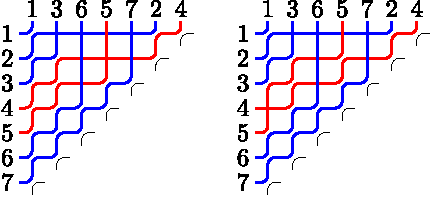
\includegraphics[scale=.9]{pipeDreams}
	}
	\caption{Two pipe dreams of~$\pipeDreams(1365724)$ connected by a flip (exchanging an elbow with the crossing on the two red pipes~$3$ and~$4$).}
	\label{fig:pipeDreams}
\end{figure}

Two pipe dreams are related by a \defn{flip} if they define the same permutation of the pipes and only differ by the position of a cross and an elbow. An elbow~$e$ in a pipe dream~$P$ is \defn{flippable} if the two pipes passing through elbow~$e$ have a crossing~$c$, and the flip exchanges the elbow~$e$ with the cross~$c$. See \fref{fig:pipeDreams}. The flip is \defn{increasing} if the elbow~$e$ is weakly south-west of the crossing~$c$. For example, the flip of \fref{fig:pipeDreams} is increasing from left to right.

The \defn{contact graph} of a pipe dream~$P$ is the directed graph~$P\contact$ with one node for each pipe of~$P$ and one arc for each elbow of~$P$ connecting the north-west path to the south-east path of the elbow\footnote{We have reversed the usual orientation conventions to suit better our purposes, in particular in Section~\ref{subsec:insertionAlgorithm}.}. We see equivalently the contact graph~$P\contact$ as a graph on the pipes of~$P$ or on the integers~$[n]$. We say that a pipe dream~$P$ is \defn{acyclic} if its contact graph~$P\contact$ is (no oriented cycle). We then denote by~$\contactLess{P}$ the transitive closure of the contact graph of~$P$. For~$\omega \in \fS_n$, we denote by~$\acyclicPipeDreams(\omega)$ the set of acyclic pipe dreams of~$\pipeDreams(\omega)$.
% We let~$\acyclicPipeDreams_n \eqdef \bigsqcup_{\omega \in \fS_n} \acyclicPipeDreams(\omega)$ and~$\acyclicPipeDreams \eqdef \bigsqcup_{n \in \N} \acyclicPipeDreams_n$.
%\vincent{Add contact graphs to \fref{fig:pipeDreams}.}


%%%%%%%%%%%%%%%%%%%%%%%%%%%%%%%%%%%%%%

\subsection{Reversing pipe dreams}
\label{subsec:reversingPipeDreams}

We say that a pipe dream~$P \in \pipeDreams_n$ is \defn{reversing} if it fixes the first pipe and reverses the order of the remaining pipes, \ie if~$\omega_P = [1, n, n-1, \dots, 2]$ (in one-line notation). We denote by~$\reversingPipeDreams_n$ the reversing pipe dreams of~$\pipeDreams_n$. As observed by different authors~\cite{Woo, PilaudPocchiola, Pilaud-these, Stump}, the pipe dreams of~$\reversingPipeDreams_n$ belong to the Catalan family. \fref{fig:bijection} illustrates explicit bijections between the pipe dreams of~$\reversingPipeDreams_n$, the binary trees on $n$ vertices, and the triangulations of a convex $(n+2)$-gon.

\begin{figure}[h]
	\centerline{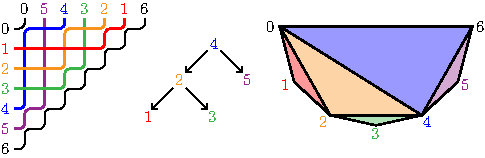
\includegraphics[scale=1.3]{dualiteTriangulation}}
	\caption{The bijection between reversing pipe dreams (left), binary trees (middle) and triangulations (right).}
	\label{fig:bijection}
\end{figure}

More precisely, the map which sends an elbow in row~$i$ and column~$j$ of the triangular shape to the diagonal~$[i,n+1-j]$ of the~$(n+2)$-gon provides the following correspondence:
\begin{center}
\begin{tabular}{r@{$\quad\longleftrightarrow\quad$}l}
pipe dream~$P \in \reversingPipeDreams_n$ & triangulation~$P\duality$ of the $(n+2)$-gon, \\
$i$th pipe of~$P$ & $i$th triangle of~$P\duality$ (with central vertex~$i$), \\
elbows of~$P$ & diagonals of~$P\duality$, \\
crosses of~$P$ & common bisectors between triangles of~$P\duality$, \\
contact graph of~$P$ & dual binary tree of~$P\duality$, \\
elbow flips in~$P$ & diagonal flips in~$P\duality$.
\end{tabular}
\end{center}

\begin{remark}
All reversing pipe dreams are acyclic. Indeed, there contact graphs are (oriented) binary trees, which are certainly acyclic.
\end{remark}

%%%%%%%%%%%%%%%%%%%%%%%%%%%%%%%%%%%%%%

\subsection{Subword complexes}
\label{subsec:subwordComplexes}

Pipe dreams are a very particular family of the family of subword complexes. Consider a Coxeter system~$(W,S)$, where~$W$ is a finite Coxeter group and~$S$ is the set of simple reflections of~$W$. We denote by~$e$ (resp.~$\wo$) the identity (resp.~longest element) of~$W$. Let~$Q \eqdef q_1 \dots q_m \in S^*$ be a word on the alphabet formed by the simple generators of~$W$ and~$w \in W$. The \defn{subword complex}~$\subwordComplex(Q,w)$ is the simplicial complex whose ground set~$[m]$ are the positions in~$Q$ and whose facets are the complements of the reduced expressions for~$w$ in~$Q$.

It is known that~$\subwordComplex(Q,w)$ is either a ball or a sphere, in particular it is a pseudomanifold (with or without boundary). The flip graph of~$\subwordComplex(Q,w)$ is the graph whose vertices are the facets of~$\subwordComplex(Q,w)$ and whose edges are the ridges of~$\subwordComplex(Q,w)$. If~$F,F'$ are two adjacent facets with~$F \ssm \{p\} = F' \ssm \{p'\}$, we say that the flip is \defn{increasing} when~$p < p'$. The increasing flip graph was studied in particular in~\cite{PilaudStump-ELlabelings}. It is known to be acyclic, and its transitive closure is an EL-shellable poset (see~\cite{PilaudStump-ELlabelings} for the precise definition and references).

There is also a notion of acyclicity for subword complexes. It is based on the notion of \defn{root configuration}~$\Roots(F)$ of a facet~$F$ of~$\subwordComplex(Q,w)$. We skip the details and refer to~\cite{CeballosLabbeStump, PilaudStump-brickPolytope} for details. The facet~$F$ is \defn{acyclic} if its root configuration is pointed (meaning that it generates a pointed cone).

\begin{example}
Consider the symmetric group~$\fS_{n+1}$ generated by the set of simple transpositions $\set{\tau_i}{i \in [n]}$ where~$\tau_i \eqdef (i \; i+1)$.
For a permutation~$\omega \in \fS_{n+1}$, the pipe dreams of~$\pipeDreams(\omega)$ correspond to the facets of the subword complex~$\subwordComplex(Q,\omega)$ with~$Q = \tau_1, \tau_2, \dots, \tau_n, \tau_1, \tau_2, \dots, \tau_{n-1}, \dots, \tau_1, \tau_2, \tau_1$. % The notions of flips, increasing flips and acyclic pipe dreams transpose in the world of subword complexes.
\end{example}

\begin{example}
For any Coxeter group~$W$ and any Coxeter element~$c \in W$ (a product of all generators of~$S$ in a given arbitrary order), let~$\wo(c)$ denote the $c$-sorting word of~$\wo$ (see \cite{Reading-CambrianLattices} for details). Extending the observation of Section~\ref{subsec:reversingPipeDreams}, it was shown in~\cite{CeballosLabbeStump} that the subword complex~$\subwordComplex(c\wo(c), \wo)$ is isomorphic to the cluster complex of type~$W$. In particular, the increasing flip graph is the Hasse diagram of the $c$-Cambrian lattice of~\cite{Reading-CambrianLattices}.
\end{example}

In contrast to the previous example, consider the word~$Q = \tau_1 \tau_2 \tau_3 \tau_2 \tau_1 \tau_2 \tau_3 \tau_2 \tau_1$ on the simple generators of the symmetric group~$\fS_4$ and the subword complex~$\subwordComplex(Q,\wo)$. Note that all facets in this subword complex are acyclic. It is shown in~\cite[Rem.~5.12]{PilaudStump-brickPolytope} that its increasing flip poset is not a lattice. This shows that neither the increasing flip poset, nor the acyclic increasing flip poset are lattices in general, even in type~$A$. In this note, we investigate the case of acyclic pipe~dreams.

%%%%%%%%%%%%%%%%%%%%%%%%%%%%%%%%%%%%%%

\subsection{Elementary properties of pipe dreams}
\label{subsec:elementaryProperties}

We gather in this section some elementary properties of pipe dreams needed later.

\begin{lemma}
\label{lem:horiVertCrossings}
For any pipe dream~$P \in \pipeDreams(\omega)$, the pipe~$j$ of~$P$ (which enters at row~$j$ and exits at column~$\omega^{-1}(j)$) crosses
\begin{itemize}
\item vertically the pipes~$i$ such that~$i < j$ while~$\omega^{-1}(i) > \omega^{-1}(j)$,
\item horizontally the pipes~$k$ such that~$j < k$ while~$\omega^{-1}(j) > \omega^{-1}(k)$.
\end{itemize}
\end{lemma}

\begin{proof}
For~$i < j$, if~$\omega^{-1}(i) > \omega^{-1}(j)$, then the pipes~$i$ and~$j$ have to cross exactly once, while if~$\omega^{-1}(i) < \omega^{-1}(j)$ the pipes~$i$ and~$j$ cannot cross. The same argument applies for~${k > j}$.
\end{proof}

\begin{lemma}
\label{lem:countingElbows}
For any pipe dream~$P \in \pipeDreams(\omega)$, the pipe~$j$ (which enters at row~$j$ and exits at column~$\omega^{-1}(j)$) has precisely
\begin{itemize}
\item $\noninversions{\omega}{j}$ many \se{} elbows\!\SEelbow{}
\item $1+\noninversions{\omega}{j}$ many \nw{} elbows~\WNelbow{}
\item $j-1-\noninversions{\omega}{j}$ vertical crossings~\NScross
\item $\omega^{-1}(j)-1-\noninversions{\omega}{j}$ horizontal crossings~\WEcross
\end{itemize}
where~$\noninversions{\omega}{j} \eqdef |\set{i \in [n]}{i < j \text{ and } \omega^{-1}(i) < \omega^{-1}(j)}|$.
\end{lemma}

\begin{proof}
Pipe~$j$ enters at row~$j$ and exits at column~$\omega^{-1}(j)$, so that it passes through~$j+\omega^{-1}(j)-1$ grid points. By Lemma~\ref{lem:horiVertCrossings}, it has~$|\set{i \in [n]}{i < j \text{ and } \omega^{-1}(i) > \omega^{-1}(j)}| = j-1-\noninversions{\omega}{j}$ vertical crossings and~$|\set{k \in [n]}{j < k \text{ and } \omega^{-1}(j) > \omega^{-1}(k)}| = \omega^{-1}(j)-1-\noninversions{\omega}{j}$ horizontal crossings. The~$1+2\,\noninversions{\omega}{j}$ remaining grid points along the pipe~$j$ are thus alternating north-west elbows and south-east elbows.
\end{proof}

\begin{lemma}
\label{lem:characterizationPipeDreams}
A collection~$P$ of~$n$ pipes pairwise disjoint except at crossing and elbows and such that for each~$j \in [n]$, the pipe~$j$ enters at row~$j$, exits at column~$\omega^{-1}(j)$, and has~$\noninversions{\omega}{j}$ \se{} elbows is a pipe dream of~$\pipeDreams(\omega)$.
\end{lemma}

\begin{proof}
The argument is similar to the previous lemma. Observe first that the pipe~$j$ must cross the paths~$i$ such that~$i < j$ and~$\omega^{-1}(i) > \omega^{-1}(j)$ and the paths~$k$ such that~$j < k$ and~$\omega^{-1}(j) > \omega^{-1}(k)$. Moreover, it has~$\noninversions{\omega}{j}$ \se{} elbows and thus~$1+\noninversions{\omega}{j}$ \nw{} elbows. This already exhausts all~$j+\omega^{-1}(j)-1$ grid points of~$j$. Therefore, the pipe~$j$ can only cross at most once any other pipe.
\end{proof}

\begin{lemma}
\label{lem:rectangle}
Let~$P$ be a pipe dream and~$p,q$ be pipes of~$P$. If there is a elbow of~$p$ weakly north-west of a elbow~$q$, then~$p \contactLess{} q$ (\ie there is an oriented path from~$p$ to~$q$ in the contact graph~$P\contact$ of~$P$).
\end{lemma}

\begin{proof}
Let~$x$ (reps.~$y$) be the location of a elbow of~$p$ (resp.~$q$) such that~$x$ is weakly north-west of~$y$. We proceed by induction on the grid distance from~$x$ to~$y$. If they coincide, then~$p$ and~$q$ share a elbow, so that there is an edge from~$p$ to~$q$ in~$P\contact$. Otherwise, let~$r$ be the pipe of~$P$ with a south-east elbow at~$x$ ($r$ is either the pipe~$p$ itself, or there is an edge from~$p$ to~$r$ in~$P\contact$) and~$s$ be the pipe of~$P$ with a north-west elbow at~$y$ ($s$ is either the pipe~$q$ itself, or there is an edge from~$s$ to~$q$ in~$P\contact$). Let~$R$ be the axis-parallel rectangle with elbows~$x$ and~$y$. Since~$r$ and~$s$ cross at most once, at least one of them has an additional elbow along the sides of~$R$. Assume for instance that~$r$ has an elbow at~$x'$. Then~$x'$ is still weakly northwest of~$y$ and $x',y$ are strictly closer than~$x,y$. By induction, there is a path from~$r$ to~$s$ in~$P\contact$, and thus a path form~$p$ to~$q$.
\end{proof}

Note that the reciprocal assertion of Lemma~\ref{lem:rectangle} is false.

%%%%%%%%%%%%%%%%%%%%%%%%%%%%%%%%%%%%%%
%%%%%%%%%%%%%%%%%%%%%%%%%%%%%%%%%%%%%%
%%%%%%%%%%%%%%%%%%%%%%%%%%%%%%%%%%%%%%

\section{Three equivalent partitions}
\label{sec:partitions}

Remember that the \defn{weak order} on~$\fS_n$ is defined as the inclusion order of inversions, where an inversion of~$\pi \in \fS_n$ is a pair of values~$i, j \in \N$ such that~$i < j$ while~$\pi^{-1}(i) > \pi^{-1}(j)$. Fix a permutation~$\omega \in \fS_n$, and let~$[e, \omega] \eqdef \set{\pi \in \fS_n}{\pi \le \omega}$ denote the weak order interval between the identity~$e$ and~$\omega$.

%%%%%%%%%%%%%%%%%%%%%%%%%%%%%%%%%%%%%%

\subsection{Linear extensions of contact graphs}
\label{subsec:linearExtensions}

Consider an acyclic pipe dream~$P$. Recall that we denote by~$\contactLess{P}$ the transitive closure of the contact graph~$P\contact$ of~$P$. We denote by~$\linearExtensions(P)$ the set of linear extensions of~$P\contact$ (\ie $\pi \in \linearExtensions(P)$ if and only if~$\pi^{-1}(i) < \pi^{-1}(j)$ for all~$i \to j$ in~$P\contact$). We often say abusively that the permutations of~$\linearExtensions(P)$ are linear extensions of~$P$. In this section, we prove certain structural properties of~$\linearExtensions(P)$. The following definitions of weak order intervals and weak order interval posets are connected in the Proposition~\ref{prop:WOIP} proved by A.~Bjorner and M.~Wachs~\cite{BjornerWachs}, see also~\cite{ChatelPilaudPons}.

\begin{definition}
\label{def:WOIP}
A \defn{weak order interval (WOI)} is a subset~$[\tau, \tau']$ of~$\fS_n$ consisting of all permutations~$\sigma \in \fS_n$ such that~$\tau \le \sigma \le \tau'$ in weak order. A \defn{weak order interval poset (WOIP)} is a poset~$\less$ on~$[n]$ such that for all~$a < b < c$,
\[
a \less c \implies a \less b \text{ or } b \less c 
\qquad\text{and}\qquad
a \more c \implies a \more b \text{ or } b \more c.
\]
\end{definition}

\begin{proposition}[\protect{\cite[Thm.~6.8]{BjornerWachs}}]
\label{prop:WOIP}
The WOIs are the sets of linear extensions of WOIPs:
\begin{enumerate}[(i)]
\item the WOI~$[\tau, \tau']$ is the set of linear extensions of the WOIP obtained as the transitive closure of the relations~$i \less j$ for all non coinversions~$i,j$ of~$\tau$ and~$i \more j$ for all coinversions~$i,j$~of~$\tau'$;
\item the linear extensions of a WOIP~$\less$ is the WOI~$[\tau,\tau']$, where~$\tau$ and~$\tau'$ are respectively the greedy and antigreedy linear extensions of~$\less$.
\end{enumerate}
\end{proposition}

We use this characterization to prove the following statement.

\begin{proposition}
\label{prop:intervals}
For any pipe dream~$P \in \acyclicPipeDreams(\omega)$, the set~$\linearExtensions(P)$ is an interval of the weak order.
\end{proposition}

\begin{proof}
We just need to show that the poset~$\contactLess{P}$ satisfies the WOIP condition.
Consider~$a < b < c$ such that~$a \contactLess{P} c$. If~$\omega^{-1}(a) < \omega^{-1}(b)$, we know from Lemma~\ref{lem:rectangle} that~$a \contactLess{P} b$. Similarly, if~$\omega^{-1}(b) < \omega^{-1}(c)$, we have~$b \contactLess{P} c$. We can therefore assume that~$\omega^{-1}(a) > \omega^{-1}(b) > \omega^{-1}(c)$. Assume moreover that~$a \contactLess{T} c$. Decompose the triangular shape into three regions: the region~$A$ of all points located south-west of the first elbow of the pipe~$b$ of~$P$, the region~$B$ of all points located north-west or south-east of an elbow of the pipe~$b$ of~$P$, and the region~$C$ of all points located north-east of the last elbow of the pipe~$b$ of~$P$. Since~$a \contactLess{T} c$, there is a path~$\pi$ form the entering point of the pipe~$a$ of~$P$ to the exiting point of the pipe~$c$ of~$P$ which travels along the pipes and the elbows of~$P$. Since~$a < b < c$, the path~$\pi$ starts in region~$A$ and ends in region~$C$, so that it necessarily passes from region~$A$ to region~$C$. Since the north-east corner of~$A$ is located south-west of the south-west corner of~$C$, this forces an elbow~$e$ of~$\pi$ to lie in region~$B$. Lemma~\ref{lem:rectangle} then ensures that either~$a \contactLess{T} b$ (if~$e$ is above the pipe~$b$), or~$b \contactLess{T} c$ (if~$e$ is below the pipe~$b$). The proof is similar if~$a \contactMore{T} c$.
\end{proof}

In the next two statements, we show that the sets~$\linearExtensions(P)$ partition an interval of the weak order.

\begin{lemma}
\label{lem:interval}
For any linear extension~$\pi$ of a pipe dream~$P \in \pipeDreams(\omega)$, we have~$\pi \le \omega$ in weak order.
\end{lemma}

\begin{proof}
Consider a non-inversion of~$\omega$, \ie~$(i,j) \in [n]^2$ such that~$i < j$ and~$\omega^{-1}(i) < \omega^{-1}(j)$. Since~$i < j$ and~$\omega^{-1}(i) < \omega^{-1}(j)$, the pipes~$i$ and~$j$ do not cross. Therefore, the path~$j$ passes south-east of any elbow of the path~$i$. This shows that~$i \contactLess{P} j$ by Lemma~\ref{lem:rectangle}. Therefore, $\pi^{-1}(i) < \pi^{-1}(j)$ for any linear extension~$\pi$ of~$P$. In other words, $(i,j)$ is also a non-inversion of~$\pi$. We conclude that all linear extensions \mbox{of~$P$ are smaller than~$\omega$ in weak order}.
\end{proof}

\begin{proposition}
\label{prop:partition}
The collection~$\set{\linearExtensions(P)}{P \in \acyclicPipeDreams(\omega)}$ forms a partition of the interval~$[e,\omega]$ of the weak order.
\end{proposition}

\begin{proof}
\vincent{There are other methods to prove this without using the sweeping algorithm... We will actually do this for arbitrary subword complexes.}
By Lemma~\ref{lem:interval}, all linear extensions belong to the interval~$[e,\omega]$. 

We now show that~$\linearExtensions(P) \cap \linearExtensions(P') = \varnothing$ for any two distinct acyclic pipe dreams~$P, P' \in \pipeDreams(\omega)$. For this, we show that we can reconstructing a pipe~$P$ knowing a linear extension~$\pi \in \linearExtensions(P)$. For this, we sweep the pipe dream in any perturbation of the \nw{} direction (meaning that we sweep the grid in any order such that each point is swept before all points weakly \nw of~$p$). When we sweep a vertex~$v$ of the grid, we see a pipe~$p$ arriving horizontally at~$v$ and a pipe~$q$ arriving vertically at~$v$. If~$p > q$, then $p$ and~$q$ already crossed before, so we have no choice but imposing an elbow at~$v$. If~$p < q$, there are three situations:
\begin{itemize}
\item if~$\pi^{-1}(p) > \pi^{-1}(q)$ then~$p$ and~$q$ cannot touch (otherwise $\pi$ would not be a linear extension of~$P$), so that we have no choice but imposing a crossing~at~$v$,
\item if~$\omega^{-1}(p) < \omega^{-1}(q)$, then~$p$ and~$q$ cannot cross (otherwise~$P$ would not be a pipe dream of~$\pipeDreams(\omega)$), so that we have no choice but imposing a contact at~$v$,
\item if~$\pi^{-1}(p) < \pi^{-1}(q)$ and~$\omega^{-1}(p) > \omega^{-1}(q)$, then we have again two situations;
	\begin{itemize}
	\item If $q$ needs to go straight north, then we have no choice but imposing a crossing at~$v$,
	\item Otherwise, we have no choice but imposing an elbow at~$v$. Indeed, if there is a crossing at~$v$, then Lemma~\ref{lem:rectangle} ensures that~$q$ will be below~$p$ in~$P\contact$, so that~$\pi$ would not be a linear extension of~$P$.
	\end{itemize}
\end{itemize}


%Several arguments could be invoked, as for example the insertion algorithm discussed in Section~\ref{subsec:insertionAlgorithm}. We prefer here to recall from~\cite{PilaudPocchiola} that one can reconstruct a pipe dream~$P$ by sweeping the triangular shape in any slight perturbation of the north-east direction. When we sweep a vertex~$v$ of the grid, we see a pipe~$p$ arriving horizontally at~$v$ and a pipe~$q$ arriving vertically at~$v$. If~$p > q$, then $p$ and~$q$ already crossed before, so we have no choice but imposing an elbow at~$v$. If~$p < q$, there are two situations:
%\begin{itemize}
%\item if~$p \not\contactLess{P} q$ then~$p$ and~$q$ cannot touch, so that we have no choice but imposing a crossing~at~$v$,
%\item if~$\omega^{-1}(p) < \omega^{-1}(q)$, then~$p$ and~$q$ cannot cross, so that we have no choice but imposing a contact at~$v$,
%\item if~$p \contactLess{P} q$ and~$\omega^{-1}(p) > \omega^{-1}(q)$, then we have again two situations;
%	\begin{itemize}
%	\item If $q$ needs to go straight north, then we have no choice but imposing a crossing at~$v$,
%	\item Otherwise, we have no choice but imposing an elbow at~$v$. \qedhere
%	\end{itemize}
%\end{itemize}

To conclude the proof, we need to show that any permutation of~$[e,\omega]$ is a linear extension of some pipe dream~$P \in \acyclicPipeDreams(\omega)$. This is done using an insertion algorithm presented next.
\end{proof}

%%%%%%%%%%%%%%%%%%%%%%%%%%%%%%%%%%%%%%

\subsection{Insertion algorithm}
\label{subsec:insertionAlgorithm}

We now define a surjective map from the permutations of~$[e, \omega]$ to the pipe dreams of~$\acyclicPipeDreams(\omega)$. This map, adapted from~\cite{Pilaud-BrickAlgebra}, is obtained by an insertion process similar to the insertion in binary search trees. 
%To properly describe this insertion algorithm, we introduce additional notations.
We now describe this insertion algorithm, which is illustrated in \fref{fig:insertionAlgorithm}. 

Consider a given permutation~$\pi \eqdef \pi(1) \dots \pi(n)$ (written in one-line notation) in~$[e, \omega]$. We start from the empty triangular shape and insert the pipes~$\pi(1), \dots, \pi(n)$ one by one in the order of the permutation~$\pi$ as \nw{} as possible. In other words, at step~$t$, we consider the set~$X_t$ of free \nw{} elbows in the rectangle~$[\pi(t)] \times [\omega^{-1}(\pi(t))]$. The pipe inserted at step~$t$ then starts in row~$\pi(t)$, ends in column~$\omega^{-1}(\pi(t))$, covers each elbow of~$X_t$ with a \se{} elbow, and adds just one new free \nw{} elbow in between any two consecutive elbows of~$X_t$. We denote the resulting pipe dream by~$\insertion{\pi}{\omega}$. See \fref{fig:insertionAlgorithm}.

\begin{figure}[b]
	\centerline{
		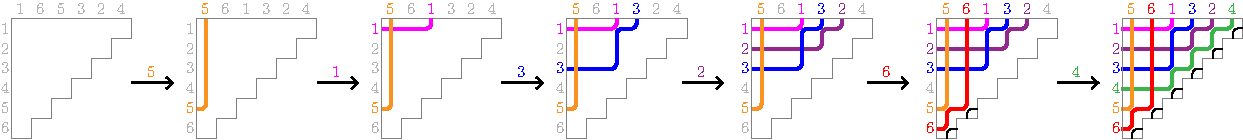
\includegraphics[scale=.9]{insertion}
	}
	\caption{The insertion~$\insertion{513264}{561324}$.}
	\label{fig:insertionAlgorithm}
\end{figure}

We need to argue that this algorithm indeed creates a pipe dream of~$\acyclicPipeDreams(\omega)$. To see it, we observe that the following invariant is maintained throughout the algorithm.

\begin{lemma}
\label{lem:rectangleInsertionAlgorithm}
At each step~$t$ of the insertion algorithm, we have
\[
|X_t| = \big| \bigset{s < t}{\pi(s) < \pi(t) \text{ and } \omega^{-1}\big( \pi(s) \big) < \omega^{-1}\big( \pi(t) \big)} \big|.
\]
\vincent{Note that this is independent of~$\pi$... This can be seen from Lemma~\ref{lem:interval}.}
\end{lemma}

\begin{proof}
Fix~$t \in [n]$. At the beginning of the algorithm, there is no \se{} elbow in the rectangle~$R_t \eqdef [\pi(t)] \times [\omega^{-1}(\pi(t))]$. At each step~$s < t$, we have inserted a new pipe~$\pi(s)$ which enters at~$\pi(s)$ and exits at~$\omega^{-1}\big( \pi(s) \big)$. We conclude by considering the four possible cases:
\begin{itemize}
\item If~$\pi(s) < \pi(t)$ and~$\omega^{-1}\big( \pi(s) \big) < \omega^{-1}\big( \pi(t) \big)$, then the pipe~$\pi(s)$ is completely contained in the rectangle~$R_t$. Since the pipe~$\pi(s)$ has one more \nw{} elbow than \se{} elbow, its insertion creates a new free \nw{} elbow in the rectangle~$R_t$.
\item If~$\pi(s) < \pi(t)$ and~$\omega^{-1}\big( \pi(s) \big) > \omega^{-1}\big( \pi(t) \big)$, then the pipe~$\pi(s)$ enters and exits the rectangle~$R_t$ with an horizontal step, so that it has as many \nw{} and \se{} elbows in~$R_t$, and its insertion does not modify the number of free \nw{} elbows in the rectangle~$R_t$.
\item If~$\pi(s) > \pi(t)$ and~$\omega^{-1}\big( \pi(s) \big) < \omega^{-1}\big( \pi(t) \big)$, then the pipe~$\pi(s)$ enters and exits the rectangle~$R_t$ with a vertical step, so that it has as many \nw{} and \se{} elbows in~$R_t$, and its insertion does not modify the number of free \nw{} elbows in the rectangle~$R_t$.
\item If~$\pi(s) > \pi(t)$ and~$\omega^{-1}\big( \pi(s) \big) > \omega^{-1}\big( \pi(t) \big)$, then setting~$i = \pi(t)$ and~$j = \pi(s)$, we have~$i < j$ and~$\pi^{-1}(i) > \pi^{-1}(j)$ while~$\omega^{-1}(i) < \omega^{-1}(j)$, which contradicts our assumption that~$\pi \not< \omega$ in weak order. \qedhere
\end{itemize}
\end{proof}

\begin{corollary}
For any~$\pi \le \omega$, the insertion algorithm creates a pipe dream~$\insertion{\pi}{\omega}$ of~$\pipeDreams(\omega)$.
\end{corollary}

\begin{proof}
The algorithm constructs a collection~$P$ of $n$ pairwise disjoint pipes except at crossings and elbows. For each~$t \in [n]$, the pipe~$\pi(t)$ enters at~$\pi(t)$, exits at~$\omega^{-1}\big( \pi(t) \big)$, and has 
\[
\big| \bigset{s < t}{\pi(s) < \pi(t) \text{ and } \omega^{-1}\big( \pi(s) \big) < \omega^{-1}\big( \pi(t) \big)} \big| = \noninversions(\omega, \pi(t))
\]
many $\se$ elbows by Lemma~\ref{lem:rectangleInsertionAlgorithm} and since~$\pi < \omega$ in weak order. We thus conclude the proof by a direct application of Lemma~\ref{lem:characterizationPipeDreams}.
\vincent{Maybe we should argue that the pipes remain in the triangle.}
\end{proof}

\begin{proposition}
\label{prop:fibersInsertion}
For any pipe dream~$P \in \acyclicPipeDreams(\omega)$,  the permutations~$\pi \le \omega$ such that~$\insertion{\pi}{\omega} = P$ are precisely the linear extensions of the contact graph~$P\contact$ of~$P$. In particular, $\insertion{\cdot}{\omega}$ is a surjection from~$[e, \omega]$ to~$\acyclicPipeDreams(\omega)$.
\end{proposition}

\begin{proof}
By construction of the insertion algorithm, all \se{} elbows of the pipe~$\pi(t)$ inserted at step~$t$ are in contact with \nw{} elbows of pipes~$\pi(s)$ inserted at steps~$s < t$. In other words, all edges in the contact graph of~$\insertion{\pi}{\omega}$ are of the form~$\pi(s) \to \pi(t)$ for some~$s < t$. It follows that the permutation~$\pi$ is a linear extension of~$\insertion{\pi}{\omega}$. Reciprocally, consider a linear extension~$\pi$ of a pipe dream~$P$. Then~$\insertion{\pi}{\omega}$ and~$P$ have a common linear extension~$\pi$, so that~$\insertion{\pi}{\omega} = P$ by Proposition~\ref{prop:partition}.
\end{proof}

In other words, the sets~$\set{\linearExtensions(P)}{P \in \acyclicPipeDreams(\omega)}$ are the fibers of the surjective insertion map~$\insertion{\cdot}{\omega}$. Note that this concludes the proof of the surjectivity left open in Proposition~\ref{prop:partition}.

%%%%%%%%%%%%%%%%%%%%%%%%%%%%%%%%%%%%%%

\subsection{Pipe dream congruence}
\label{subsec:pipeDreamCongruence}

We now characterize the sets of linear extensions of pipe dreams in terms of a rewriting rule. We write the permutations of~$\fS_n$ as words in one-line notation.

\begin{definition}
\label{def:congruence}
For any permutation~$\omega \in \fS_n$, the \defn{pipe dream congruence} is the equivalence relation~$\equiv_\omega$ on the interval~$[e,\omega]$ of the weak order defined as the transitive closure of the rewriting rule~$U ac V \equiv_\omega U ca V$ if and only if
\[
|\set{b \in U}{a < b < c \text{ and } \omega^{-1}(a) > \omega^{-1}(b) > \omega^{-1}(c)}| \ge |\set{b < a}{\omega^{-1}(b) < \omega^{-1}(c)}|,
\]
\vincent{Note that $b \in U$ on the right hand side by Lemma~\ref{lem:interval}.}
where~$a, b, c$ are elements of~$[n]$ while~$U, V$ are (possibly empty) words on~$[n]$. The letters~$b \in U$ such that~$a < b < c$ while~$\omega^{-1}(a) > \omega^{-1}(b) > \omega^{-1}(c)$ are called \defn{pipe dream congruence witnesses} for the exchange of~$a$ and~$c$.
\vincent{Another option to write this is $d \ge u$ where $d \eqdef \set{b \in U}{b > a}$ and~$u \eqdef \set{b \in U}{\omega^{-1}(b) < \omega^{-1}(c)}$. Or $dr \ge \ell u$ where $dr \eqdef \set{b \in U}{b > a \text{ and } \omega^{-1}(b) > \omega^{-1}(c)}$ and~$\ell u \eqdef \set{b \in U}{b < a \text{ and } \omega^{-1}(b) < \omega^{-1}(c)}$.}
\end{definition}

\begin{proposition}
\label{prop:congruence}
For any~$\pi, \pi' \in [e,\omega]$, we have~${\pi \equiv_\omega \pi' \!\iff\! \insertion{\pi}{\omega} = \insertion{\pi'}{\omega} \!\iff\! \pi}$~and~$\pi'$ are linear extensions of a same pipe dream.
\end{proposition}

\begin{proof}
By Proposition~\ref{prop:fibersInsertion}, each fiber of~$\insertion{\cdot}{\omega}$ gathers the linear extensions of a pipe dream of~$\pipeDreams(\omega)$. Since the set of linear extensions of a poset is connected by simple transpositions, we just need to show that~$\pi \equiv_\omega \pi' \!\iff\! \insertion{\pi}{\omega} = \insertion{\pi'}{\omega}$ for any two permutations~$\pi = UacV$ and~$\pi' = UcaV$ of~$[e,\omega]$ which differ by the inversion of two consecutive values.

Let~$t = \pi^{-1}(a) = \pi'{-1}(c)$. At step~$t$ of the algorithm presented in the previous section, we have inserted the word~$U$. At that moment, let~$X_t$ (resp.~$X'_t$, resp~$Y_t$) denote the set of free \nw{} elbows in the rectangle~$[a] \times [\omega^{-1}(a)]$ (resp.~$[c] \times [\omega^{-1}(c)]$, resp.~$[a] \times [\omega^{-1}(c)]$). Applying the same argument as in Lemma~\ref{lem:rectangleInsertionAlgorithm}, we have
\begin{gather*}
|Y_t| = \max\big( |\set{b \in U}{b < a \text{ and } \omega^{-1}(b) < \omega^{-1}(c)}| \hspace{5cm} \\ \hspace{5cm} - |\set{b \in U}{a < b < c \text{ and } \omega^{-1}(a) > \omega^{-1}(b) > \omega^{-1}(c)}|, 0\big).
\end{gather*}
It follows that~$U ac V \equiv_\omega U ca V \iff |Y_t| = 0$. However, $Y_t = 0$ if and only if all elbows of~$X_t$ are in~$[a] \times [\omega^{-1}(c), \omega^{-1}(a)]$ and all elbows of~$X'_t$ are in~$[a,c] \times [\omega^{-1}(c)]$. The latter is equivalent to the fact that the insertion of~$a$ and~$c$ commute. We conclude that
\[
U ac V \equiv_\omega U ca V \iff \insertion{UacV}{\omega} = \insertion{UcaV}{\omega},
\]
which concludes the proof since the set of linear extensions of a poset is connected by simple transpositions.
\end{proof}

\begin{proposition}
\label{prop:patternAvoiding}
The minimal (resp.~maximal) permutations in the partition
\(
{[e,\omega] = \bigsqcup_{P \in \acyclicPipeDreams(\omega)} \linearExtensions(P)}
\)
are the permutations avoiding the patterns~$b_1 - \cdots - b_k - ca$ (resp.~$b_1 - \cdots - b_k - ac$) where $k = |\set{b < a}{\omega^{-1}(b) < \omega^{-1}(c)}|$.
\end{proposition}

\begin{proof}
This is an immediate consequence of Proposition~\ref{prop:congruence}: a permutation~$\pi$ is minimal (resp.~maximal) in its $\equiv_\omega$-congruence class if and only if it contains no consecutive exchangeable entries~$ca$ (resp.~$ac$) with~$a < c$.
\end{proof}

To sum up, there are three equivalent ways to partition the interval~$[e,\omega]$ of the weak order:
\vincent{In fact, we should write 4 different ways, the last one being the sweeping algorithm.}
\begin{itemize}
\item by the sets of linear extensions~$\linearExtensions(P)$ of all pipe dreams of~$\acyclicPipeDreams(\omega)$,
\item by the fibers of the insertion map~$\insertion{\cdot}{\omega}$,
\item by the classes of the pipe dream congruence~$\equiv_\omega$.
\end{itemize}

%%%%%%%%%%%%%%%%%%%%%%%%%%%%%%%%%%%%%%
%%%%%%%%%%%%%%%%%%%%%%%%%%%%%%%%%%%%%%
%%%%%%%%%%%%%%%%%%%%%%%%%%%%%%%%%%%%%%

\section{Lattice of acyclic pipe dreams}
\label{sec:latticeAcyclicPipeDreams}

Based on the result of the previous section, we now show that the pipe dream congruence~$\equiv_\omega$ is a lattice congruence of the interval~$[e,\omega]$ of weak order for any~$\omega \in \fS_n$. We extend the proof of~\cite{Pilaud-BrickAlgebra} which treated the particular case of~$\omega = [1, \dots, k, n-k, \dots, k+1, n-k+1, \dots, n]$.

%%%%%%%%%%%%%%%%%%%%%%%%%%%%%%%%%%%%%%

\subsection{Lattice congruences and lattice quotients}
\label{subsec:latticeCongruences}

We first remind the reader with the definition of these congruences and refer to~\cite{Reading-LatticeCongruences, Reading-CambrianLattices} for further details.

An \defn{order congruence} is an equivalence relation~$\equiv$ on a poset~$P$ such that:
\begin{enumerate}[(i)]
\item Every equivalence class under~$\equiv$ is an interval of~$P$.
\item The projection~$\projDown : P \to P$ (resp.~$\projUp : P \to P$), which maps an element of~$P$ to the minimal (resp.~maximal) element of its equivalence class, is order preserving.
\end{enumerate}
The \defn{quotient}~$P/{\equiv}$ is a poset on the equivalence classes of~$\equiv$, where the order relation is defined by~$X \le Y$ in~$P/{\equiv}$ iff there exists representatives~$x \in X$ and~$y \in Y$ such that~$x \le y$ in~$P$. The quotient~$P/{\equiv}$ is isomorphic to the subposet of~$P$ induced by~$\projDown(P)$ (or equivalently by~$\projUp(P)$).

If moreover~$P$ is a finite lattice, then~$\equiv$ is a automatically \defn{lattice congruence}, meaning that it is compatible with meets and joins: for any~$x \equiv x'$ and~$y \equiv y'$, we have~$x \meet y \equiv x' \meet y'$ and~$x \join y \equiv x' \join y'$. The poset quotient~$P/{\equiv}$ then inherits a lattice structure where the meet~$X \meet Y$ (resp.~the join~$X \join Y$) of two congruence classes~$X$ and~$Y$ is the congruence classe of~$x \meet y$ (resp.~of~$x \join y$) for arbitrary representatives~$x \in X$ and~$y \in Y$.

%Lattice quotient of the weak order.
%Connection to the increasing flip poset.

%%%%%%%%%%%%%%%%%%%%%%%%%%%%%%%%%%%%%%

\subsection{The pipe dream congruence is a lattice congruence}
\label{subsec:proofCongruence}

We are now ready to prove the main statement of this note. Recall that an interval in a lattice is itself a lattice, so that the weak order on~$[e,\omega]$ has a lattice structure.

\begin{theorem}
For any permutation~$\omega \in \fS_n$, the pipe dream congruence~$\equiv_\omega$ is a lattice congruence of the interval~$[e,\omega]$ of the weak order.
\end{theorem}

\begin{proof}
We already observed in Proposition~\ref{prop:intervals} that the $\equiv_\omega$-congruence classes are intervals of the weak order. We therefore just need to show that~$\tau < \tau'$ implies~$\min(C) < \min(C')$ and $\max(C) < \max(C')$ for any two permutations~$\tau, \tau' \in [e,\omega]$ from distinct $\equiv_\omega$-congruence classes~$C,C'$. We only prove the result for the maximums, the proof for the minimums being similar. We first observe that we can assume that~$\tau' = \tau s_i$ for some simple transposition~${s_i = (i \;\, i+1)}$ which is not a descent of~$\tau$. The proof then works by induction on the weak order distance between~$\tau$ and~$\max(C)$. If~$\tau = \max(C)$, the result is immediate as~$\max(C) = \tau < \tau' \le \max(C')$. Otherwise, consider a permutation~$\sigma$ in~$C$ covering~$\tau$ in weak order. We write~$\sigma = \tau s_j$, and $s_j$ is not a descent of~$\tau$. We now distinguish four cases, according to the relative positions of~$i$ and~$j$:
\begin{enumerate}[(1)]
\item If~$i > j+1$, we have~$\tau = UabVcdW$, $\tau' = UabVdcW$ and~$\sigma = UbaVcdW$ for some letters~$a < b$ with~$\omega^{-1}(a) > \omega^{-1}(b)$, some letters~$c < d$ with~$\omega^{-1}(c) > \omega^{-1}(d)$ and some words~$U,V,W$. Define~$\sigma' \eqdef \tau s_i s_j = \tau' s_j = \sigma s_i = UbaVdcW$. Since~$\tau \equiv_\omega \sigma$, there exist $k = |\set{u < a}{\omega^{-1}(u) < \omega^{-1}(b)}|$ $\equiv_\omega$-congruence witnesses~$u_1, \dots, u_k$ in the word~$U$, with~$a < u_\ell < b$ and~$\omega^{-1}(a) > \omega^{-1}(u_\ell) > \omega^{-1}(c)$ for all~$\ell \in [k]$. These letters are also $\equiv_\omega$-congruence witnesses for the equivalence~$\tau' \equiv_\omega \sigma'$. Moreover, $\sigma < \sigma'$ since~$c < d$.
\item If~$i = j+1$, we have~$\tau = UabcW$, $\tau' = UacbW$ and~$\sigma = UbacW$ for some letters~${a < b < c}$ with~$\omega^{-1}(a) > \omega^{-1}(b) > \omega^{-1}(c)$ (since~$\tau < \omega$ in weak order by asumption) and some words~$U,W$. Define~$\sigma' \eqdef \tau s_i s_j s_i = \tau' s_j s_i = \sigma s_i s_j = UcbaW$. Since~$\tau \equiv_\omega \sigma$, there exist $k = |\set{u < a}{\omega^{-1}(u) < \omega^{-1}(b)}|$ $\equiv_\omega$-congruence witnesses~$u_1, \dots, u_k$ in the word~$U$, with ${a < u_\ell < b}$ and~$\omega^{-1}(a) > \omega^{-1}(u_\ell) > \omega^{-1}(c)$ for all~$\ell \in [k]$. Since~$b < c$ and~$\omega^{-1}(b) > \omega^{-1}(c)$, these letters are also $\equiv_\omega$-congruence witnesses for the equivalences~${\tau' \equiv_\omega \tau' s_j \equiv_\omega \tau' s_j s_i = \sigma'}$. (Moreover, note that there are indeed enough witnesses for the equivalence~$\tau' \equiv_\omega \tau' s_j$ since ${k = |\set{u < a}{\omega^{-1}(u) < \omega^{-1}(b)}| \ge |\set{u < a}{\omega^{-1}(u) < \omega^{-1}(c)}|}$). Finally, since~$a < b < c$, we have~$\sigma < \sigma'$.
\item If~$i = j-1$, we proceed similarly as in Situation~(2).
\item If~$i < j-1$, we proceed similarly as in Situation~(1).
\end{enumerate}
In all cases, we have~$\tau \equiv_\omega \sigma < \sigma' \equiv_\omega \tau'$. Since~$\sigma$ is closer to~$\max(C)$ than~$\tau$, we obtain that ${\max(C) < \max(C')}$ by induction hypothesis.
\end{proof}

%%%%%%%%%%%%%%%%%%%%%%%%%%%%%%%%%%%%%%

\subsection{Lattice of acyclic pipe dreams}
\label{subsec:proofCongruence}

Finally, we need to show that the lattice quotient~$[e,\omega]/\equiv_\omega$ is isomorphic to the increasing flip poset on~$\acyclicPipeDreams(\omega)$. This is the purpose of the following statement.

\begin{proposition}
For any pipe dreams~$P, P' \in \acyclicPipeDreams(\omega)$, the following assertions are equivalent:
\begin{enumerate}[(i)]
\item $P < P'$ in the increasing flip poset on~$\acyclicPipeDreams(\omega)$,
\item there exist linear extensions~$\pi$ of~$P$ and~$\pi'$ of~$P'$ such that~$\pi < \pi'$ in weak order,
\item the minimal (resp.~max) linear extensions~$\pi$ of~$P$ and~$\pi'$ of~$P$ satisfy~$\pi < \pi'$ in weak order.
\end{enumerate}
\end{proposition}

\begin{proof}
Consider two distinct acyclic pipe dreams~$P, P' \in \acyclicPipeDreams(\omega)$ and their $\equiv_\omega$-congruence~classes~$C, C'$. If there exist representatives~$\pi = UijV \in C$ and~$\pi' = UjiV \in C'$ which are adjacent in weak order, then~$P = \insertion{\pi}{\omega}$ and~$P' = \insertion{\pi'}{\omega}$ differ by the flip of the first/last elbow between the pipes~$i$ and~$j$, by definition of the map~$\insertion{\cdot}{\omega}$. Conversely, if~$P$ and~$P'$ differ by the flip of the first/last elbow between the pipes~$i$ and~$j$, then $i$ and~$j$ are connected in the contact graph~$P\contact$, so that there exists a linear extension~$\pi = UijV$ of~$P\contact$ where~$i$ and~$j$ are consecutive. Let~$\pi' = UjiV$ be the permutation obtained by the switch of~$i$ and~$j$ in~$\pi$. By definition of the map~$\insertion{\cdot}{\omega}$, the pipe dream~$\insertion{\pi'}{\omega}$ is obtained by flipping the first elbow between the pipes~$i$ and~$j$ in~$\insertion{\pi}{\omega}$. The representatives~$\pi \in C$ and~$\pi' \in C'$ are thus adjacent in weak order. This proves that~$\insertion{\cdot}{\omega}$~induces an isomorphism from the quotient lattice of the interval~$[e,\omega]$ of the weak order by the $\equiv_\omega$-congruence to the increasing flip order on acyclic pipe dreams of~$\acyclicPipeDreams(\omega)$. In turn, since the $\equiv_\omega$-congruence is a lattice congruence, this quotient lattice is isomorphic to the subposet of the weak order induced by the minimal (resp.~maximal) elements of the classes. See~\cite{Reading-LatticeCongruences, Reading-CambrianLattices} for further details on quotient lattices.
\vincent{I am not sure anymore that this proof is correct. At least this could require more explanations.}
\end{proof}

\begin{corollary}
For any permutation~$\omega \in \fS_n$, the increasing flip poset on~$\acyclicPipeDreams(\omega)$ is a lattice.
\end{corollary}


%%%%%%%%%%%%%%%%%%%%%%%%%%%%%%%%%%%%%%
%%%%%%%%%%%%%%%%%%%%%%%%%%%%%%%%%%%%%%
%%%%%%%%%%%%%%%%%%%%%%%%%%%%%%%%%%%%%%

\section{Canopy}
\label{sec:canopy}

Recall that the \defn{canopy} of a binary tree~$T$ with~$n$ internal nodes is the sign sequence~${\canopy{T} \in \{{-},{+}\}^{n-1}}$ defined by~$\canopy{T}_i = {-}$ if the $(i+1)$st leaf of~$T$ is a left leaf and~$\canopy{T}_i = {+}$ if the $(i+1)$st leaf of~$T$ is a right leaf. Equivalently, $\canopy{T}_i = -$ if the node~$i$ of~$T$ is above the node~$i+1$ of~$T$ and~$\canopy{T}_i = +$ otherwise. This map was already used by J.-L.~Loday in~\cite{LodayRonco, Loday}, but the name ``canopy'' was coined by X.~Viennot~\cite{Viennot}.
% The binary search tree insertion map and the canopy map factorize the recoil map: $\surjectionBrickZono[] \circ \surjectionPermBrick[] = \surjectionPermZono[]$. This combinatorial fact can also be understood on the geometry of the normal fans of the permutahedron, the associahedron and the cube, see Section~\ref{subsec:normalFans}.

Before introducing the canopy, let us define the $\omega$-recoils. For this, consider the graph~$G(\omega)$ with vertex set~$[n]$ and edge set
\[
\bigset{ij}{i < j \text{ and } j-i \le |\set{k < i}{\omega^{-1}(k) < \omega^{-1}(j)}|}.
\]
Let~$\acyclicOrientations(\omega)$ denote the set of acyclic orientations of~$G(\omega)$.

\begin{definition}
The \defn{$\omega$-recoil scheme} of a permutation~$\pi \in [e,\omega]$ is the orientation~${\recoils{\pi}{\omega} \in \acyclicOrientations(\omega)}$ where for all~$i < j \in [n]$ such that~$j-i \le |\set{k < i}{\omega^{-1}(k) < \omega^{-1}(j)}|$, the edge~$ij$ is oriented~$i \to j$ if~$\pi^{-1}(i) < \pi^{-1}(j)$ and~$j \to i$ if~$\pi^{-1}(j) < \pi^{-1}(i)$. We call \defn{$\omega$-recoil map} the map~$\recoils{\cdot}{\omega} : [e,\omega] \to \acyclicOrientations(\omega)$.
\end{definition}

\begin{remark}
The fiber of an acyclic orientation~$O \in \acyclicOrientations(\omega)$ under the $\omega$-recoil map~$\recoils{\cdot}{\omega}$ are the linear extensions of~$O$ in~$[e,\omega]$.
\end{remark}

We now define a generalization of the canopy map for pipe dreams in~$\acyclicPipeDreams(\omega)$. To ensure that Definition~\ref{def:canopy} is valid, we need the following simple observation on comparisons of ``close'' pipes in a pipe dream.

\begin{lemma}
\label{lem:canopy}
If~$i < j$ satisfy~$j-i \le |\set{k < i}{\omega^{-1}(k) < \omega^{-1}(j)}|$, then the pipes~$i$ and~$j$ in any acyclic pipe dream~$P \in \acyclicPipeDreams(\omega)$ are comparable~for~$\contactLess{P}$.
\end{lemma}

\begin{proof}
If pipes~$i$ and~$j$ were incomparable in~$\contactLess{P}$, there would be two $\equiv_\omega$-congruent permutations~$UijV \equiv_\omega UjiV$. However, the assumption contradicts the definition of the $\equiv_\omega$-conguence in Definition~\ref{def:congruence}.
\end{proof}

\begin{definition}
\label{def:canopy}
The \defn{canopy} of a pipe dream~$P \in \acyclicPipeDreams(\omega)$ is the orientation~$\canopy{P} \in \acyclicOrientations(\omega)$ where for all~$i < j \in [n]$ such that~$j-i \le |\set{k < i}{\omega^{-1}(k) < \omega^{-1}(j)}$, the edge~$ij$ is oriented~$i \to j$ if~$i \contactLess{P} j$ and~$j \to i$ if~$j \contactLess{P} i$. It indeed defines an acyclic orientation of~$G(\omega)$ by Lemma~\ref{lem:canopy}. We call \defn{canopy} the map~$\canopy{\cdot}: \acyclicPipeDreams(\omega) \to \acyclicOrientations(\omega)$.
\end{definition}

\begin{proposition}
\label{prop:latticeHomomorphisms}
The maps~$\recoils{\cdot}{\omega}$, $\insertion{\cdot}{\omega}$, and~$\canopy{\cdot}$ define the following commutative diagram of lattice homomorphisms:
\[
\begin{tikzpicture}
  \matrix (m) [matrix of math nodes,row sep=1.2em,column sep=5em,minimum width=2em]
  {
     [e,\omega]  	&								& \acyclicOrientations(\omega)	\\
					& \acyclicPipeDreams(\omega) 	&								\\
  };
  \path[->] (m-1-1) edge node [above] {$\recoils{\cdot}{\omega}$} (m-1-3);
  \path[->>] (m-1-1) edge node [below] {$\insertion{\cdot}{\omega}\qquad$} (m-2-2.west);
  \path[->] (m-2-2.east) edge node [below] {$\quad\canopy{\cdot}$} (m-1-3);
\end{tikzpicture}
\]
\end{proposition}

\begin{proof}
Consider a permutation~$\pi$ and let~$i < j \in [n]$ be such that~$j-i \le |\set{k < i}{\omega^{-1}(k) < \omega^{-1}(j)}$. Assume that the edge~$ij$ is oriented from~$i$ to~$j$. Then~$\pi^{-1}(i) < \pi^{-1}(j)$, thus the pipe~$i$ is inserted before the pipe~$j$ in~$\insertion{\pi}{\omega}$, so that~$i \contactLess{\insertion{\pi}{\omega}} j$ and there is also an arc from~$i$ to~$j$ in~$\canopy{\insertion{\pi}{\omega}}$.
\end{proof}

%%%%%%%%%%%%%%%%%%%%%%%%%%%%%%%%%%%%%%
%%%%%%%%%%%%%%%%%%%%%%%%%%%%%%%%%%%%%%
%%%%%%%%%%%%%%%%%%%%%%%%%%%%%%%%%%%%%%

\section{Future work}
\label{sec:futureWork}

\subsection{Sortability and alignement}

We should describe the minimum (or maximum) of the congruence classes of~$\equiv_\omega$ by
\begin{itemize}
\item a pattern avoiding condition, see Proposition~\ref{prop:patternAvoiding}.
\item ``$\omega$-sortability'', see~\cite{Reading-sortableElements}.
\item ``$\omega$-alignement'', see~\cite{Reading-sortableElements}.
\end{itemize}

\subsection{Other Coxeter groups}

\vincent{This part is not up-to-date.  We have new (hopefully correct) conjectures.}
All the arguments presented above should extend to type A Cambrian pipe dreams... This means that we consider the increasing flip poset of the type~$A$ subword complex~$\subwordComplex(\wo(c),\omega)$ for any Coxeter element~$c$ and any permutation~$\omega$ of~$\fS_n$. Similar arguments where already developed in~\cite{Pilaud-BrickAlgebra} for the particular case of the permutation
\[
\omega = [1, \dots, k, n-k, n-k-1, \dots, k+2, k+1, n-k+1, \dots, n].
\]
More generally, we can consider the following conjecture.

\begin{conjecture}
\label{conj:Coxeter}
For any finite Coxeter group~$W$, any Coxeter element~$c$ of~$W$, and any element~$w \in W$, the increasing flip poset on the acyclic facets of the subword complex~$\subwordComplex(\wo(c),w)$ is a lattice quotient of the interval~$[e,w]$ of the weak order on~$W$.
\end{conjecture}

Let's be a little more precise here: for an acyclic facet~$F$ of the subword complex~$\subwordComplex(\wo(c),w)$, one can consider the set~$\set{\pi \in W}{\R_{\ge 0} \pi(\Delta) \supseteq \R_{\ge 0} \Roots(F)}$, \ie the elements of~$W$ whose dual Coxeter chamber belongs to the cone generated by the root configuration of~$F$. I hope that this defines a lattice congruence of~$[e,w]$.

We should actually consider the lattice properties of the acyclic facets of~$\subwordComplex(c^k\wo(c),w)$ for any~$k$ and any~$w$. In type~$A$, this is the same as any subword complex~$\subwordComplex(c^k\wo(c),w)$ can be embedded in a bigger~$\subwordComplex(\wo(c'),w')$. In other types however it is a more general question.

\subsection{Hopf algebra}

Define an equivalence relation~$\equiv$ on intervals~$[\pi,\omega]$ of the weak order by~$[\pi,\omega] \equiv [\pi',\omega'] \iff \omega = \omega' \text{ and } \pi \equiv_\omega \pi'$. Essentially, we proved that the collection of all acyclic pipe dreams is in bijection with the equivalence classes of~$\equiv$. Now is there a Hopf algebra on intervals of the weak order such that the equivalence relation~$\equiv$ gives a subalgebra?
\vincent{I believe that this part should disappear.}

%%%%%%%%%%%%%%%%%%%%%%%%%%%%%%%%%%%%%%
%%%%%%%%%%%%%%%%%%%%%%%%%%%%%%%%%%%%%%
%%%%%%%%%%%%%%%%%%%%%%%%%%%%%%%%%%%%%%

\bibliographystyle{alpha}
\bibliography{latticePipeDreams}
\label{sec:biblio}

%%%%%%%%%%%%%%%%%%%%%%%%%%%%%%%%%%%%%%

\end{document}
